\documentclass[../../main.tex]{subfiles}
\begin{document}

\begin{flushright}
\footnotesize\textit{【自動文字起こし・要確認】}
\end{flushright}

\noindent
{\bf [解]}

\paragraph{(1)}

$P(t, t^2)$ とおく．$P$ での $y=x^2$ の接線は $y = 2tx - t^2$ だから，
\begin{align}
A\Bigl(\dfrac{t}{2}, 0\Bigr), \quad B(0, -t^2)
\end{align}
となる．したがって，
\begin{align}
\begin{cases}
g(t) = \dfrac{1}{2}\Bigl(1 - \dfrac{t}{2}\Bigr) t^2 = \dfrac{1}{4}(2-t)t^2 \\[1ex]
h(t) = \dfrac{1}{2}(2t - t^2)(1-t)
\end{cases}
\end{align}
となる．$0 < t \le 1$ のとき
\begin{align}
g(t) \le h(t) &\iff \dfrac{1}{2}(2t - t^2)(1-t) - \dfrac{1}{4}(2-t)t^2 \ge 0 \\
&\iff 2(2-t)(1-t)t - (2-t)t^2 \ge 0 \\
&\iff (2-t)t(2-3t) \ge 0 \\
&\iff 0 \le t \le \dfrac{2}{3}
\end{align}
だから，$t$ を $x$ に置き換えて，$0 < x \le \dfrac{2}{3}$ である．

\medskip
\noindent
\paragraph{(2)}

三角形の頂点が $M$ の弧上にある時，辺の延長上の点と $M$ の周囲の交点を新たな頂点とすれば，面積はより大きくなる．したがって三角形の面積が最大の時，3頂点 $\alpha, \beta, P$ は $M$ の周上にある．

$P(t, t^2)$ で $\triangle \alpha \beta P$ が $M$ の周または内部にあるから，対称性より $\alpha$ が $OC$ 上，$\beta$ が $CD$ 上にあるとして，$\alpha(a,0), \beta(1,b)$ とおくと ($y=x^2$ が下に凸より)
\begin{align}
\dfrac{t}{2} \le a \le 1, \quad 0 \le b \le 2t - t^2
\end{align}
である．以下 $t$ の値を固定して考える．

\paragraph{$1^\circ \ \dfrac{t}{2} \le a \le t$ の時}
$a$ を固定して $\triangle P \alpha \beta$ を考えると，$P\alpha$ を底辺とみれば $\beta = C$ の時高さが最大となる．
次に $\alpha$ を動かすと同じく $a = A$ で最大となる．よってこの時
\begin{align}
f(x) = \text{Area}(\triangle PAC) = g(t)
\end{align}

\paragraph{$2^\circ \ t \le a \le 1$ の時}
同様にして $f(x) = \text{Area}(\triangle PCB) = h(t)$

\medskip
$\alpha, \beta$ が同一辺上にある時も明らかに $\max \text{Area}(\triangle P\alpha\beta)$ は $g(t)$ か $h(t)$ だから，次に $t$ を動かして，
\begin{align}
f(t) = \max \{ g(t), h(t) \} = \begin{cases}
h(x) & (0 < x \le 2/3) \\
g(x) & (2/3 \le x < 1)
\end{cases}
\end{align}
増減を調べる：
\begin{align}
g'(t) = \dfrac{1}{4}(4t - 3t^2) = \dfrac{1}{4}t(4-3t) > 0 \quad \Bigl(0 < t < 1\Bigr)
\end{align}
\begin{align}
h'(t) = \dfrac{1}{2}(t^2 - 2t) + \dfrac{1}{2}(2 - 2t)(1-t) = \dfrac{1}{2}(3t^2 - 6t + 2)
\end{align}
$h'(t) = 0$ の根は $t = \dfrac{3 \pm \sqrt{3}}{3}$ である．

\begin{table}[htb]
\centering
\caption{$h(t)$ の増減表}
\begin{tabular}{c|ccccc}
$t$ & $0$ & $\dots$ & $\dfrac{3-\sqrt{3}}{3}$ & $\dots$ & $1$ \\
\hline
$h'$ & & $+$ & $0$ & $-$ & \\
\hline
$h$ & & $\nearrow$ & 極大 & $\searrow$ &
\end{tabular}
\end{table}

グラフを図示すると以下のようになる（極大値: $\dfrac{\sqrt{3}}{9}$，極小値: $\dfrac{4}{27}$）．

\begin{figure}[htb]
\centering
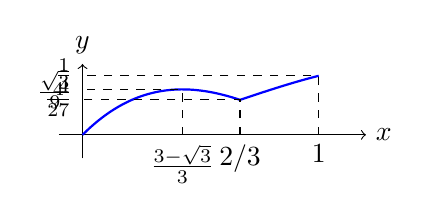
\begin{tikzpicture}[scale=3]
    \draw[->] (-0.1,0) -- (1.2,0) node[right] {$x$};
    \draw[->] (0,-0.1) -- (0,0.3) node[above] {$y$};
    
    % h(x) from 0 to 2/3
    \draw[domain=0:0.6667, smooth, variable=\x, blue, thick] plot ({\x}, {0.5*(2*\x - \x*\x)*(1-\x)});
    % g(x) from 2/3 to 1
    \draw[domain=0.6667:1, smooth, variable=\x, blue, thick] plot ({\x}, {0.25*(2-\x)*\x*\x});
    
    \draw[dashed] ({ (3-sqrt(3))/3 }, 0) node[below] {$\frac{3-\sqrt{3}}{3}$} -- ({ (3-sqrt(3))/3 }, {sqrt(3)/9}) -- (0, {sqrt(3)/9}) node[left] {$\frac{\sqrt{3}}{9}$};
    \draw[dashed] (0.6667, 0) node[below] {$2/3$} -- (0.6667, 4/27) -- (0, 4/27) node[left] {$\frac{4}{27}$};
    \draw[dashed] (1, 0) node[below] {$1$} -- (1, 0.25) -- (0, 0.25) node[left] {$\frac{1}{4}$};
\end{tikzpicture}
\caption{$y = f(x)$ のグラフ}
\end{figure}

\end{document}
